\documentclass[a4paper]{report}
\usepackage[utf8]{inputenc}
\usepackage[portuguese]{babel}
\usepackage{a4wide}
\usepackage{hyperref}
\hypersetup{pdftitle={DSL para Cadernos de Anotações em HD},
pdfauthor={Joao Teixeira, Jose Filipe Ferreira, Miguel Solino},
colorlinks=true,
urlcolor=blue,
linkcolor=black}
\usepackage{subcaption}
\usepackage[cache=false]{minted}
\usepackage{listings}
\usepackage{booktabs}
\usepackage{multirow}
\usepackage{appendix}
\usepackage{tikz}
\usepackage{authblk}
\usepackage[parfill]{parskip}
\usetikzlibrary{snakes,arrows,shapes}
\usepackage{amsmath}
\usetikzlibrary{positioning,automata,decorations.markings}

\begin{document}

\title{DSL para Cadernos de Anotações em HD \\
\large TP2 - Exercício 2 - Grupo 7}
\author{Joao Teixeira (A85504) \and Jose Filipe Ferreira (A83683) \and Miguel
Solino (A86435)}
\date{\today}

\begin{center}
    \begin{minipage}{0.75\linewidth}
        \centering
        
\includegraphics[width=0.4\textwidth]{eng.jpeg}\par\vspace{1cm}
        \vspace{1.5cm}
        \href{https://www.uminho.pt/PT}
        {\color{black}{\scshape\LARGE Universidade do Minho}} \par
        \vspace{1cm}
        \href{https://www.di.uminho.pt/}
        {\color{black}{\scshape\Large Departamento de Informática}} \par
        \vspace{1.5cm}
        \maketitle
    \end{minipage}
\end{center}

\begin{abstract}
    \begin{center}
        O objetivo deste projeto é construir um processador para cadernos de
        anotações, sendo capaz de converter um conjunto de cadernos num 
        site \textit{HTML} bem estruturado.
    \end{center}
\end{abstract}

\tableofcontents

\pagebreak

\chapter{Introdução}
Com este projeto pretende-se processar um conjunto de cadernos de anotações, com
o formato descrito no enunciado fornecido.

Para a construção de um processador capaz disto, primeiro foi escrita uma
gramática capaz de definir a DSL de \textit{caderno de anotação}. Em seguida foi
escrito um filtro de texto com recurso a \textit{FLex}, de forma a ser capaz de
fazer corresponder o texto de entrada à gramática anteriormente descrita. Para
finalizar, com recurso a \textit{yacc}, foram definidas as ações que
correspondem a cada parte da gramática, para efetuar o \textit{parsing} e
posterior criação do site \textit{HTML}.

Ao longo deste relatório iremos expor o problema, e explicar a solução
encontrada, começando por falar da arquitetura e estruturas de dados, explicando
a gramática definida e entrando em maior detalhe sobre como é efetuado o
processamendo de cada caderno. Por fim, iremos apresentar também um pequeno
manual de utilização do programa criado.

\chapter{Problema}

O programa tem que cumprir os seguintes requisitos:
\begin{itemize}
    \item Reconhecer e validar vários cadernos de anotações;
    \item Criar uma página \textit{HTML} por cada tópico, sujeito ou objeto
        presente no caderno, agrupando toda a informação respetiva ao mesmo;
    \item Incluir na página de um sujeito uma imagem sempre que apareça no
        caderno um par do tipo \textit{:x :img "img.jpg"};
    \item Ter a possibilidade de referir triplos inversos, por forma a melhorar
        a organização da informação no site criado;
\end{itemize}

\chapter{Solução}

\section{Arquitetura do Projeto}

A nossa solução divide-se em dois módulos, um correspondente ao filtro de texto,
e um correspondente à parte da gramática, armazenamento e processamento do
ficheiro de entrada e criação do site \textit{HTML}.

Quanto a estruturas de dados, numa primeira iteração do desenvolvimento apenas
existia uma lista contendo informação referente aos triplos inversos, sendo todo
o resto escrito diretamente na página correspondente ao sujeito em
processamento. 

Mas por forma a obter um aspeto mais consistente em todas as páginas
construidas, são agora armazenadas todas as informações dos triplos.
Para conseguirmos isto, criamos estruturas de dados semelhantes ao formato dos
tripos, um \textit{HashMap}, indexado por sujeito, fazendo corresponder a cada
indice, um segundo \textit{HashMap}, este indexado pela relação e contendo uma
lista de objetos.

\begin{figure}[H]
    \centering
    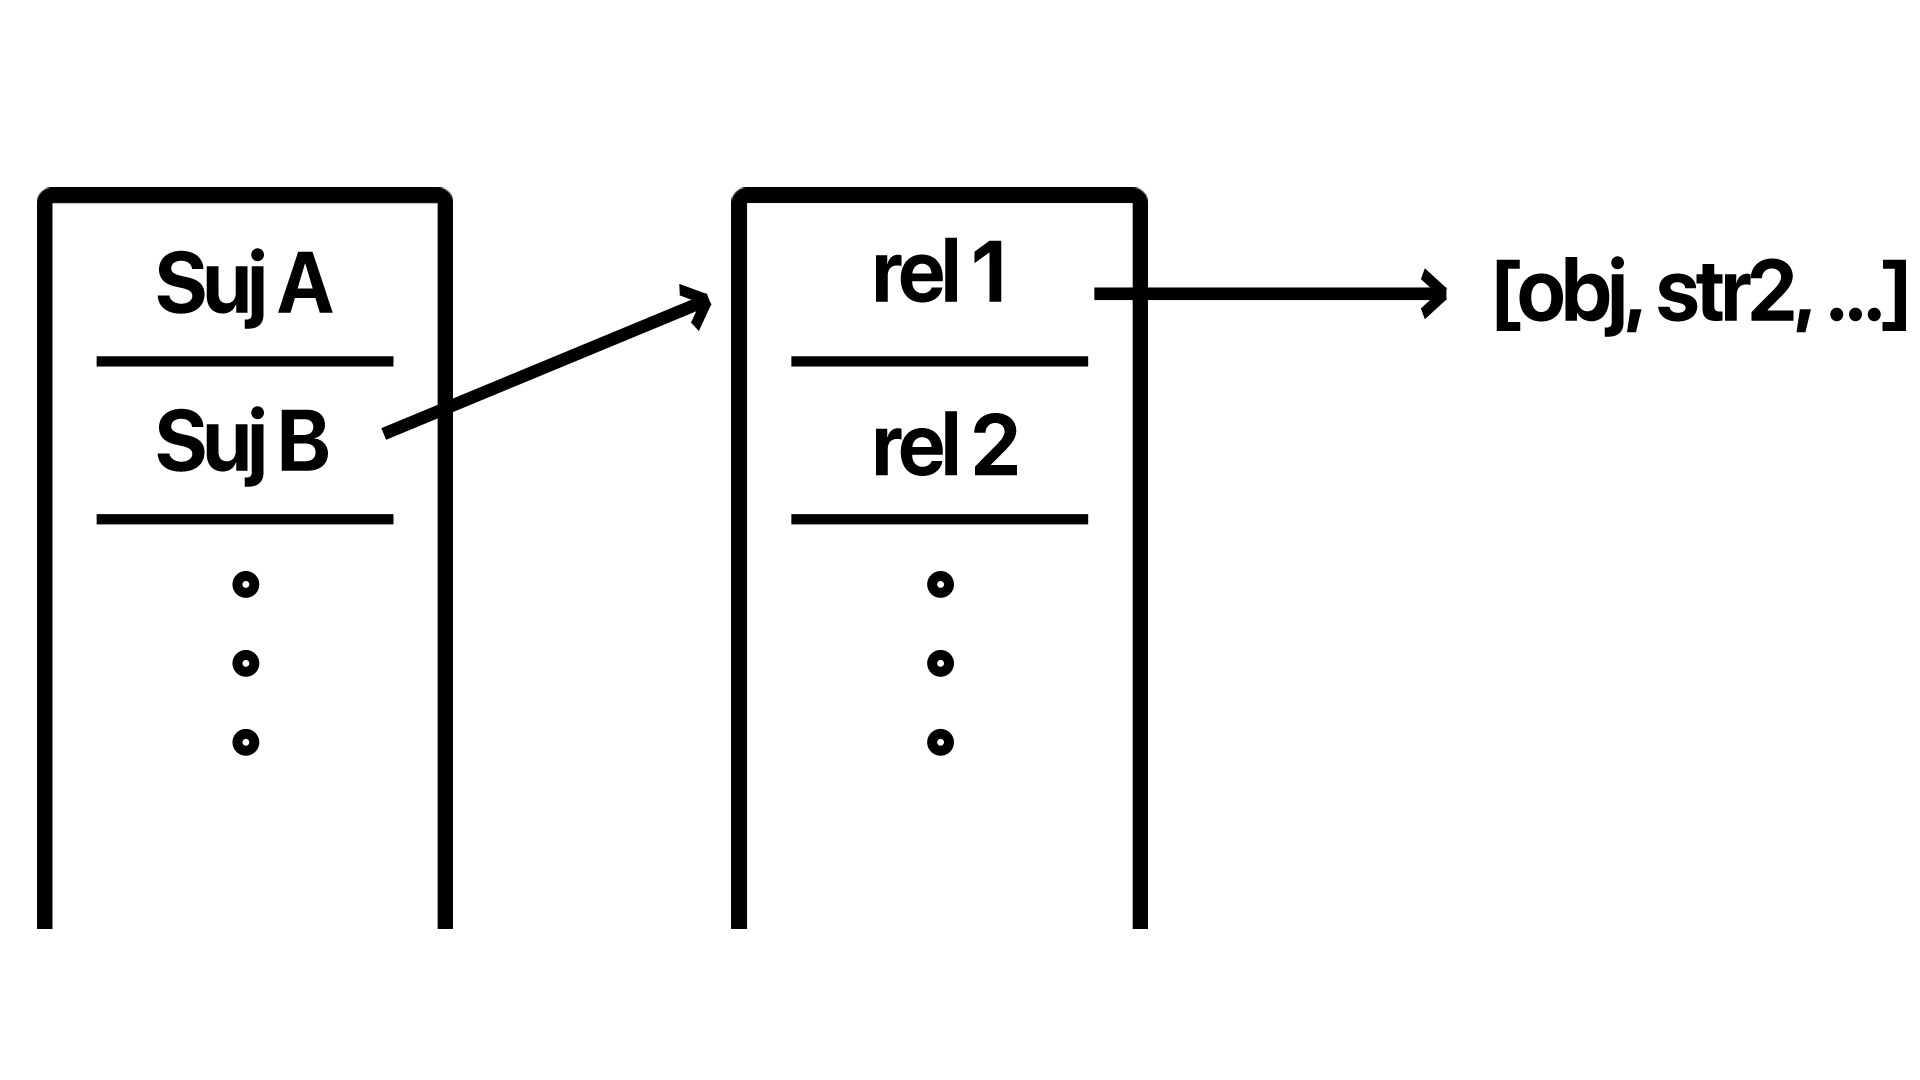
\includegraphics[width=0.88\textwidth]{data_struct.png}
    \caption{Esquema da estrutura de dados do programa}
\end{figure}

\section{Especificação da gramática}

\subsection{Símbolos terminais}

Para a especificação desta gramática, foram definidos nove símbolos terminais,
sendo a maioria marcadores ou separadores de estados (INIT, TR, IMG, MT, INV).
Os restantes correspondem a dados vindos do ficheiro de entrada, sendo estes, o
STR, que corresponde a quando um objeto de um triplo é uma string, o CONTEUDO,
correspondendo a um parágrafo do texto de um tópico, o TIT que corresponde ao
título do texto de um tópico e por fim os URI, que correpondem aos tópicos,
sujeitos ou objetos (normalmente começados por \textit{:}).

\subsection{Meta} 

Esta secção corresponde ao reconhecimento do ficheiro que contém os triplos
inversos, reconhecidos com a ajuda do simbolo terminal INV, retornado pelo flex
quando é encontrada a relação \textit{:inverseOf}.

\subsection{Conceito}

Um caderno é um conjunto de pares (Documento, Triplos), sendo a representação
de cada um deste pares um conceito. É aqui que é utilizado o simbolo terminal
TR, que marca a separação entre o Documento e os Triplos.

\subsection{Documento}

Um Documento é onde é reconhecido o texto de um conceito, e é separado em quatro
partes, um simbolo terminal INIT, que marca o ínicio de um documento, o Sujeito,
dizendo o objeto ao qual o documento se refere, um título, com o título do
texto, e o conteudo, sendo este um conjunto de parágrafos, que formam o texto em
sí.

\subsection{Triplos}

Os Triplos correspondem ao reconhecimento dos triplos em notação turtle, sendo
estes com a forma (sujeito, relação, objeto), suportando a possibilidade de por
sujeitos iguais em evidência. Na nossa gramática cada triplo, ou triplos com o
mesmo sujeito, é representado começando com um Sujeito do triplo e a uma lista
de pares explicados abaixo.

\subsection{Par}

Um Par nesta gramática corresponde a uma Relação e a uma lista de objetos e
strings, denominada de Comps. 

\subsection{Rel}

Rel corresponde às relações entre os sujietos e objetos, ao segundo elemento dos
triplos da notação turtle. Existem vários tipos de relações, existindo duas que
possuem um comportamento diferente das outras, a relação 'a' e a relação ':img'.
Numa relação do tipo 'a' os objetos correspondem ao tipo do sujeito do triplo.
Numa relação do tipo ':img' é especificada uma imagem para ser mostrada no site
\textit{HTML}, na pagína do sujeito do triplo.

\section{Processamento de um Caderno}

Para processar um caderno, constituido por vários pares (documento, triplos),
processam-se cada um dos pares.

Para processar um destes pares, começa-se por validar e tratar a parte do
documento, verificando se começa por verificar se começa pelo identificador de
início de documento, valida-se o sujeito, e cria-se a sua respetiva página
\textit{HTML} caso ainda não exista, e adiciona-se informação sobre este na
pagína do indice. Depois é processado o título do documento, escrevendo-o com a
formatação respetiva para títulos \textit{HTML} no ficheiro do sujeito. Em
seguida é processado o texto em sí, formatando-o e escrevendo-o diretamente na
página do sujeito em questão.

Depois do processamento da parte inicial do par, passa-se à parte dos triplos.
O processamento dos triplos corresponde processar recursivamente pares do tipo
(Sujeito, Pares). O processamento do sujeito decorre da forma anteriormente
explicada. Para processar os Pares, que é uma lista de pares (Rel, Comps),
percorre-se esta lista recursivamente, processando cada um dos pares
individualmente.

Para processaar um par do tipo (Rel, Comps), começamos por processar o primeiro
elemento, Rel, que corresponde ao segundo elemento dos tripos em notação turtle.
Depois de validada pelo flex, é procurada a relação inversa e guardada, para
quando forem processados os objetos presentes no terceiro e ultimo elemento dos
triplos da notação turtle, ser possível guardar de imediato nas nossas 
estruturas de dados a informação sobre não só a relação a ser processada, mas
também o seu inverso.

Por último, processamos o tipo Comps, que corresponde a uma lista de strings ou
objetos (URI). Aqui é criada uma lista guardada em memória, com todos os
elementos da relação, e guardados na estrutura de dados criada para o efeito,
já tendo em conta as relações inversas.

Processados todos os cadernos passados ao programa, é percorrida a nossa
estrutura de dados, por forma a preencher as páginas \textit{HTML} com a
respetiva informação.

\chapter{Manual de Utilização}

Este programa é de utilização simples, recebendo como argumento os cadernos a ser processado, 
podendo ser chamado desta forma: 
\verb!./turtle path_to_input_file1 path_to_input_file2!.

Para explorar o site resultante do processamento dos ficheiros de entrada, pode
abrir o ficheiro \textit{index.html} com um qualquer browser.

\chapter{Conclusão}

Para concluir, fazemos um balanço bastante positivo do projeto, conseguindo
atingir todos os requisitos definidos, conseguindo com sucesso aplicar os
conhecimentos adquiridos ao longo desta Unidade Curricular num contexto mais
prático.

\appendix

\chapter{FLex}
\lstinputlisting[basicstyle=\scriptsize\ttfamily, firstline=3]
{../filter.l}

\chapter{Yacc} \label{apx:yacc}
\lstinputlisting[basicstyle=\scriptsize\ttfamily, firstline=31, lastline=112]
{../grammar.y}

\end{document}
